
This chapter provides important artifacts related to design of our project.

\section{Software Design}

This section presents the UML class diagram and gives a brief description of each class in our system. Attributes and methods of each class and relationship among classes are clearly presented. Our project contains the following classes. All the following classes except for Static classes are derived from Django Model Class because they will be directly communicating to database and define schema of it.


\begin{figure}[h]
\centering
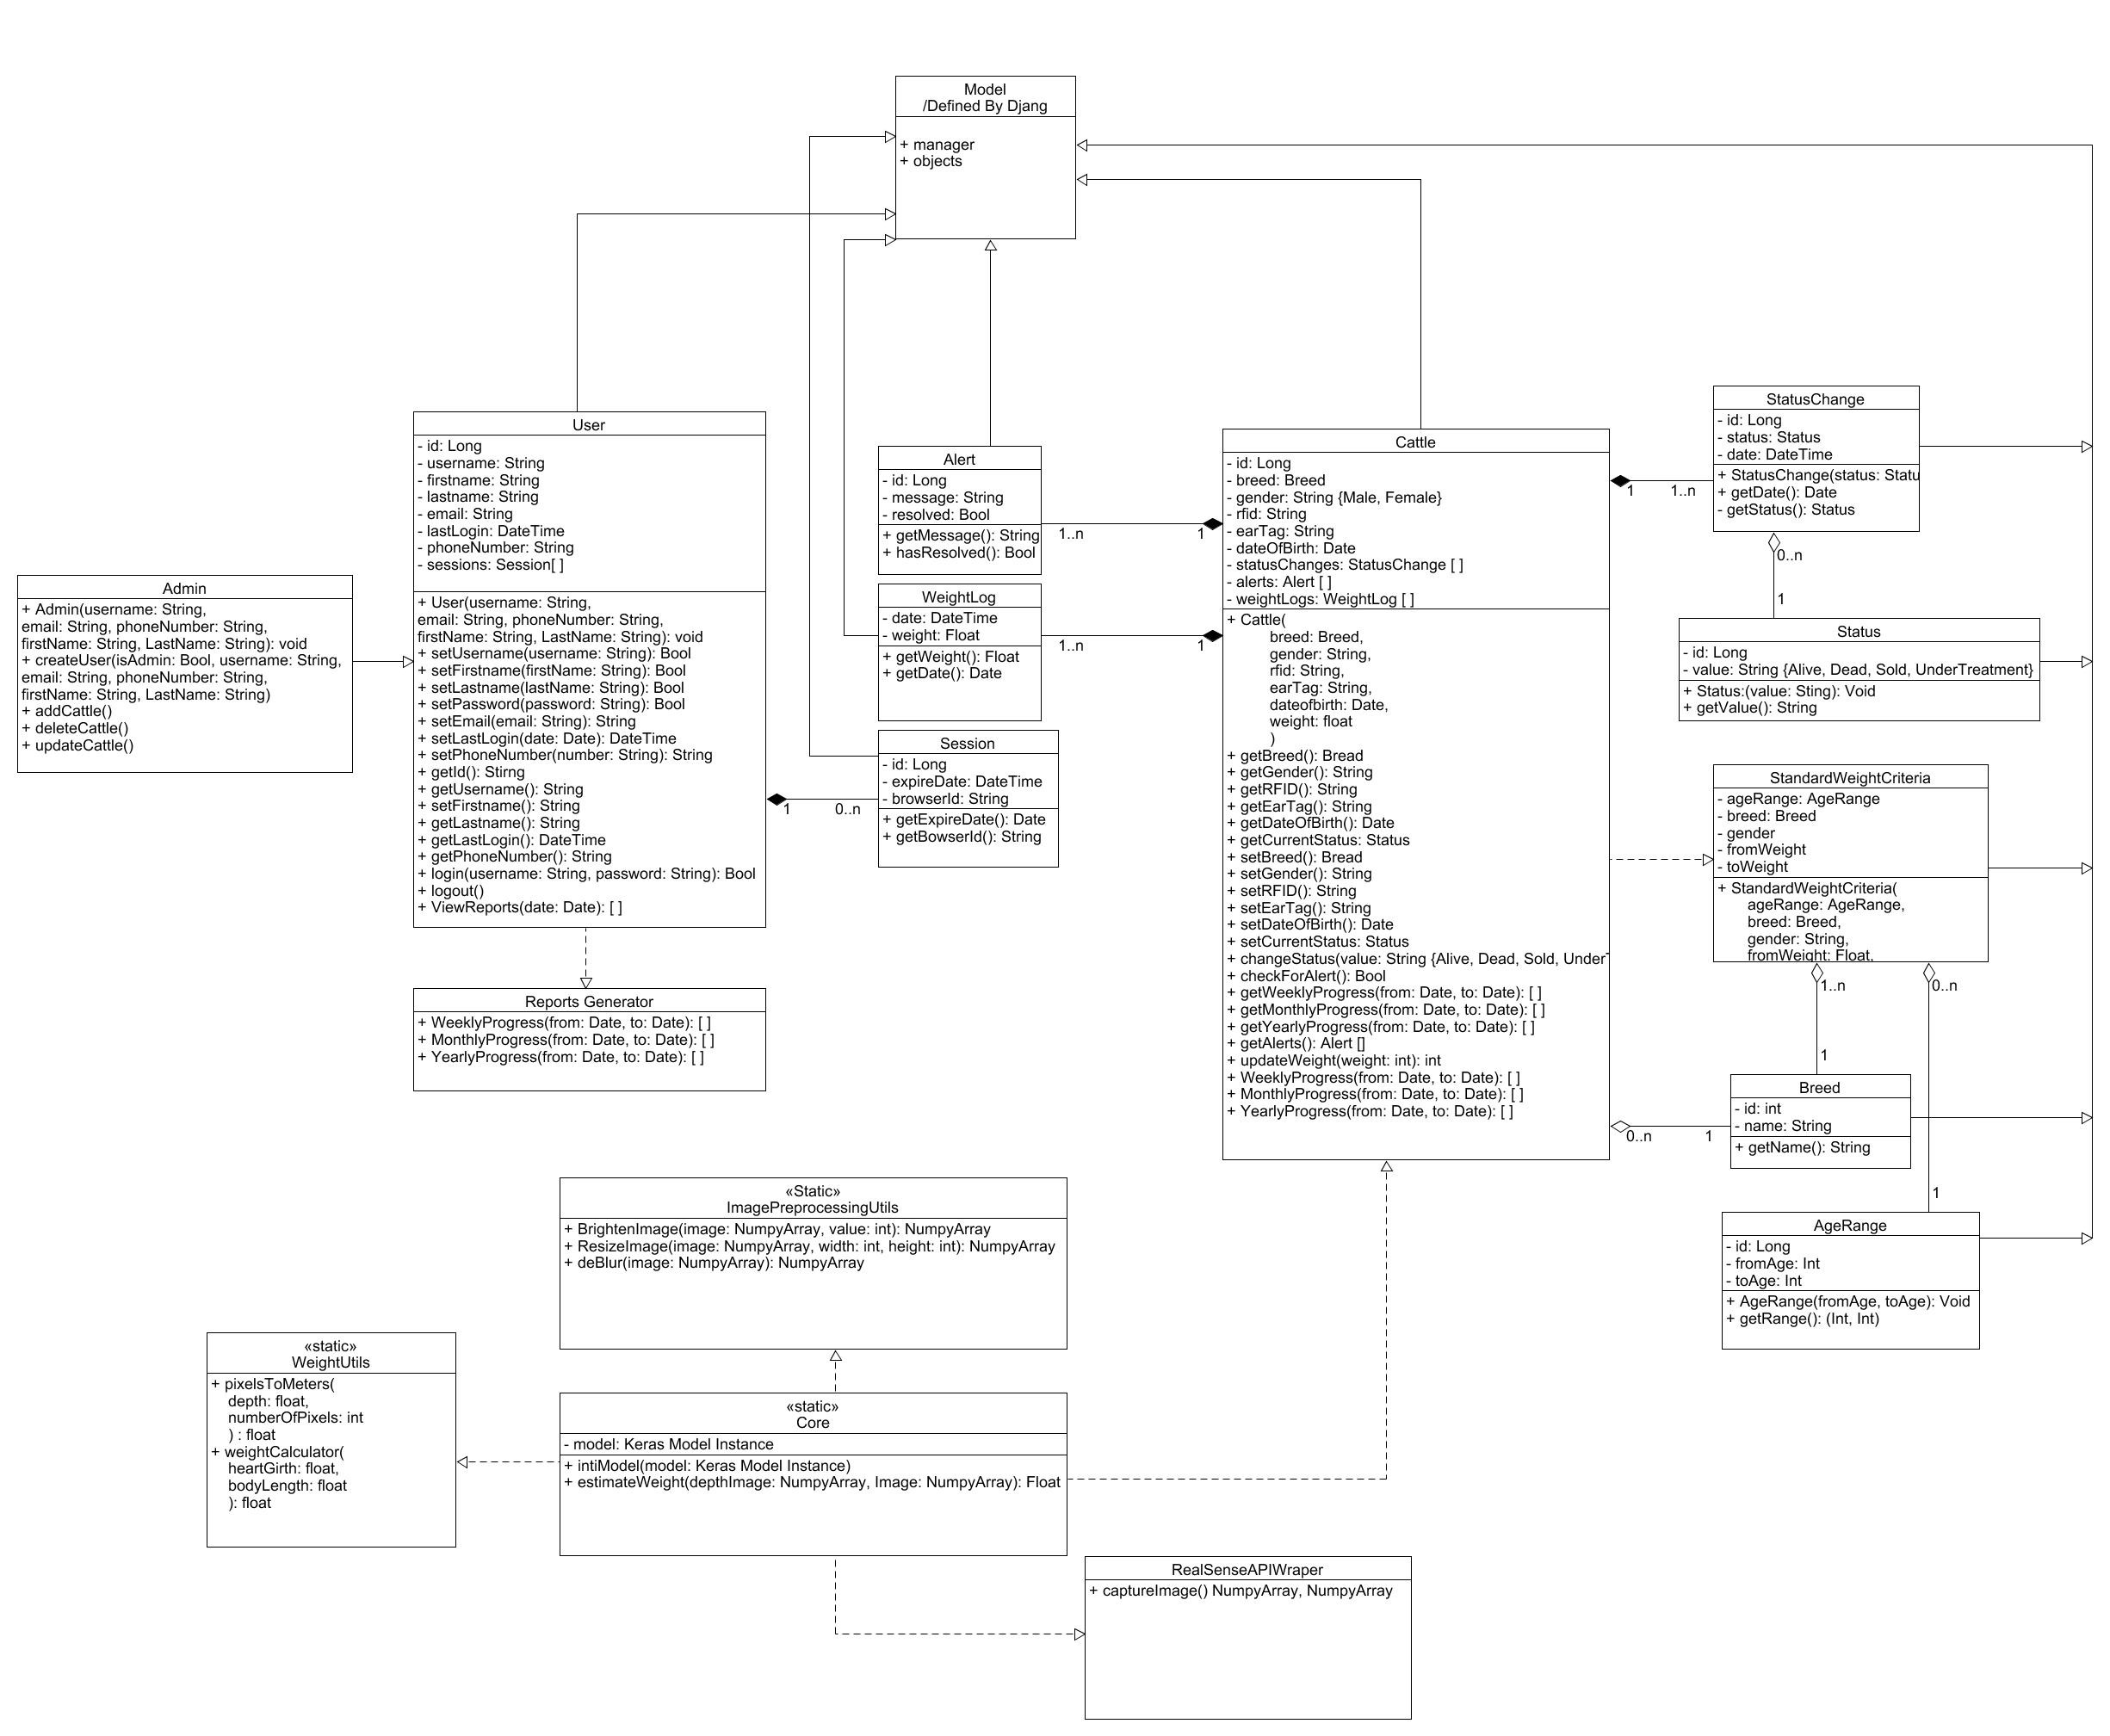
\includegraphics [scale=0.2] {FYP_UML}
\caption{Software Design Diagram (Class Diagram)}
\end{figure}


\subsection{User}
This class represents a generic user in out system. In the system there are two types of user \textbf{Admin} and \textbf{Simple User} therefore another class '\textbf{Admin}' is derived from this class. 

The class encapsulates information like \textbf{firstname, lastname, username, password, currently active session} for a perticular instance of a user.

\subsection{Admin}

This is a subclass of user which has additional access of \textbf{creating}, \textbf{updating} and deleting a users also, only the admin has access to \textbf{CRUD} operations on \textbf{Cattle}.

\subsection{Sessions}

Session encapsulates the information about a particular session of a user. User has an array of his/her currently active sessions. 

\subsection{Cattle}
This class encapsulates all details of a cattle object. some of the attributes are \textbf{rfid, earTag, dateOfBirth}. Since cattle must belong to a specific \textbf{Breed}, it store reference to the breed it belongs to. It also has some object level and some class level methods to access reports. All class methods are capitalized. While generating alerts for a cattle it is dependent on standard weight criteria.  

\subsection{Alert}
This class encapsulates details of an alert object. An alert will be generated if cattle is exceeding its \textbf{Standard Weight Criteria}.  

\subsection{Standard Weight Criteria}
This class encapsulates information about a weight criteria for a specific breed for a specific age range. 

\subsection{Age Range:}
This class encapsulates information about an age range. An Age range is a range of age which is required to define a standard weight criteria.

\subsection{Breed:}
The class encapsulates information about a breed. 

\subsection{Status}
The class encapsulates information about a Status of a cattle. Status specifies whether the cattle is under overweight, underweight, good or bad condition.

\subsection{Status Change}
This class encapsulates change in the state of a cattle at a particular instance. A Cattle object has an array of status changes in it. 

\subsection{Weight Log}
This class encapsulates information about weight change of a particular cattle object at a particular instance. A Cattle object has an array of Weight Logs in it. 

\subsection{Core (Static Class)}
This class has some static methods for weight estimation and model initiation. the classes is dependent on the static methods of other three static classes of \textbf{WeightUtils, IntelRealsenseAPIWraper, and ImagePreprocessingUtils} .


\section{Data Design}

This section presents the structure of our database that caters to persistent data storage in our project. The structure is shown as a normalized data model for relational databases. It clearly shows entities, attributes, relationships with their cardinalities, and primary and foreign keys. We have used DB designer (or any other similar data modeling tool) to build our data model.


\begin{figure}[h]
\centering
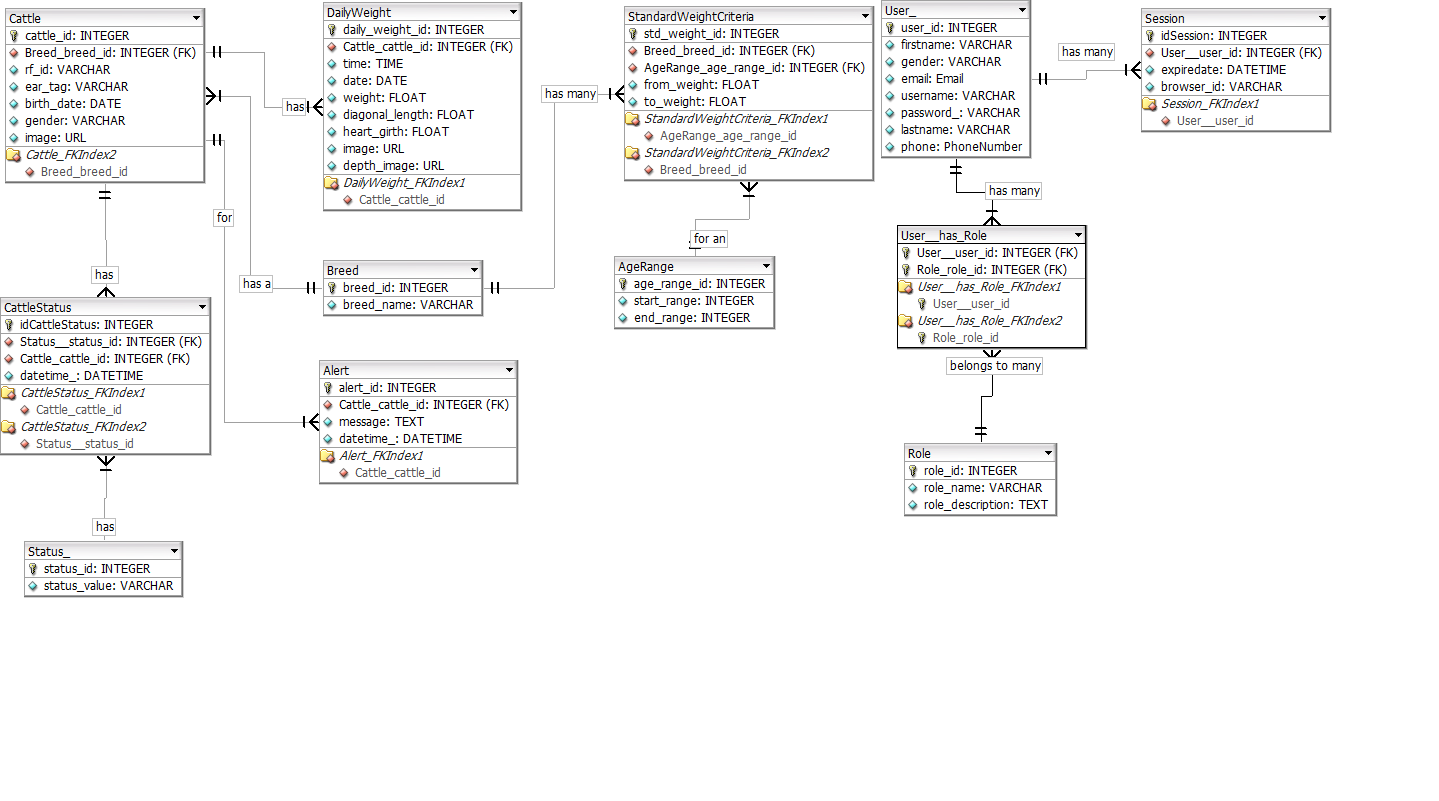
\includegraphics [scale=0.3] {erd.png}
\caption{Entity Relationship Diagram}
\end{figure}

The system has following Entities:
\subsection{User}
This represents a generic user and its attributes. 

\subsection{Session}
This represent a serverside session of a user. User and Session have a one to many relationship therefore userId is stored as foreign key in  Session. 

\subsection{Role }
Role is a generic role representation in database. User and Roles have many to many relationship therefore a middle entity \textbf{UserHasRole} is use to resolve this.

\subsection{Cattle}
This entity represents a Cattle's attributes which are stored in database.  A cattle must have a \textbf{Breed} therefore it stores BreedId as a foreign key.

\subsection{Breed}
The entity represents a breed in database. Since a breed can belong to many cattle its id is stored as foreign key in cattle's table. A breed can also have a different weight criteria based on gender and age range therefore its id is stored as foreign key in \textbf{StandardWeightCriteria} .

\subsection{Alert}
Alert are generated when an animals state is changed. Alert entity shows the attributes stored in database. Since an alert is related to a particular cattle, cattle id is stored as a foreign key in Alert. 

\subsection{Standard Weight Criteria}
Standard weight Criteria is different for each breed and gender. This entity represents its representation in database. It has a one to many relation with breed and AgeRange their ids are stored in this entity. 


\subsection{Age Range:}
An Age range is a range of age which is required to define a standard weight criteria. 

\subsection{Status}
Status specifies whether the cattle is under overweight, underweight, good or bad condition. Its id is stored for each status change for a cattle in Status Change Entity along with Cattle Id.

\subsection{Status Change}
This entity represents change in the state of a cattle at a particular instance. It stores Cattle id and State id in it. 

\subsection{Weight Log}
It represents a weight change of a particular cattle object at a particular instance.


































